%!TEX TS-program = xelatex
\documentclass[12pt, a4paper, oneside]{article}

% пакеты для математики
\usepackage{amsmath,amsfonts,amssymb,amsthm,mathtools}  
\mathtoolsset{showonlyrefs=true}  % Показывать номера только у тех формул, на которые есть \eqref{} в тексте.

\usepackage[english, russian]{babel} % выбор языка для документа
% \usepackage[utf8]{inputenc}          % utf8 кодировка

% Основные шрифты 
\usepackage{fontspec}         
\setmainfont{Linux Libertine O}  % задаёт основной шрифт документа

% Математические шрифты 
\usepackage{unicode-math}     
\setmathfont[math-style=upright]{[Neo Euler.otf]} 


%%%%%%%%%% Работа с картинками и таблицами %%%%%%%%%%
\usepackage{graphicx} % Для вставки рисунков                
\usepackage{graphics}
\graphicspath{{images/}{pictures/}}   % папки с картинками

\usepackage{wrapfig}    % обтекание рисунков и таблиц текстом

\usepackage{booktabs}   % таблицы как в годных книгах
\usepackage{tabularx}   % новые типы колонок
\usepackage{tabulary}   % и ещё новые типы колонок
\usepackage{float}      % возможность позиционировать объекты в нужном месте
\renewcommand{\arraystretch}{1.2}  % больше расстояние между строками


%%%%%%%%%% Графики и рисование %%%%%%%%%%
\usepackage{tikz, pgfplots}  % языки для графики
\pgfplotsset{compat=1.16}

\usepackage{todonotes} % для вставки в документ заметок о том, что осталось сделать
% \todo{Здесь надо коэффициенты исправить}
% \missingfigure{Здесь будет Последний день Помпеи}
% \listoftodos --- печатает все поставленные \todo'шки


%%%%%%%%%% Внешний вид страницы %%%%%%%%%%

\usepackage[paper=a4paper, top=20mm, bottom=15mm,left=20mm,right=15mm]{geometry}
\usepackage{indentfirst}    % установка отступа в первом абзаце главы

\usepackage{setspace}
\setstretch{1.15}  % межстрочный интервал
\setlength{\parskip}{4mm}   % Расстояние между абзацами
% Разные длины в LaTeX: https://en.wikibooks.org/wiki/LaTeX/Lengths

% свешиваем пунктуацию
% теперь знаки пунктуации могут вылезать за правую границу текста, при этом текст выглядит ровнее
\usepackage{microtype}

% \flushbottom                            % Эта команда заставляет LaTeX чуть растягивать строки, чтобы получить идеально прямоугольную страницу
\righthyphenmin=2                       % Разрешение переноса двух и более символов
\widowpenalty=300                     % Небольшое наказание за вдовствующую строку (одна строка абзаца на этой странице, остальное --- на следующей)
\clubpenalty=3000                     % Приличное наказание за сиротствующую строку (омерзительно висящая одинокая строка в начале страницы)
\tolerance=10000     % Ещё какое-то наказание.

% мои цвета https://www.artlebedev.ru/colors/
\definecolor{titleblue}{rgb}{0.2,0.4,0.6} 
\definecolor{blue}{rgb}{0.2,0.4,0.6} 
\definecolor{red}{rgb}{1,0,0.2} 
\definecolor{green}{rgb}{0,0.6,0} 
\definecolor{purp}{rgb}{0.4,0,0.8} 

% цвета из geogebra 
\definecolor{litebrown}{rgb}{0.6,0.2,0}
\definecolor{darkbrown}{rgb}{0.75,0.75,0.75}

% Гиперссылки
\usepackage{xcolor}   % разные цвета

\usepackage{hyperref}
\hypersetup{
	unicode=true,           % позволяет использовать юникодные символы
	colorlinks=true,       	% true - цветные ссылки
	urlcolor=blue,          % цвет ссылки на url
	linkcolor=red,          % внутренние ссылки
	citecolor=green,        % на библиографию
	breaklinks              % если ссылка не умещается в одну строку, разбивать её на две части?
}

% меняю оформление секций 
\usepackage{titlesec}
\usepackage{sectsty}

% меняю цвет на синий
\sectionfont{\color{titleblue}}
\subsectionfont{\color{titleblue}}

% выбрасываю нумерацию страниц и колонтитулы 
\pagestyle{empty}

% синие круглые бульпоинты в списках itemize 
\usepackage{enumitem}

\definecolor{itemizeblue}{rgb}{0, 0.45, 0.70}

\newcommand*{\MyPoint}{\tikz \draw [baseline, fill=itemizeblue, draw=blue] circle (2.5pt);}

\renewcommand{\labelitemi}{\MyPoint}

% расстояние в списках
\setlist[itemize]{parsep=0.4em,itemsep=0em,topsep=0ex}
\setlist[enumerate]{parsep=0.4em,itemsep=0em,topsep=0ex}


%%%%%%%%%% Свои команды %%%%%%%%%%

% Математические операторы первой необходимости:
\DeclareMathOperator{\sgn}{sign}
\DeclareMathOperator*{\argmin}{arg\,min}
\DeclareMathOperator*{\argmax}{arg\,max}
\DeclareMathOperator{\Cov}{Cov}
\DeclareMathOperator{\Var}{Var}
\DeclareMathOperator{\Corr}{Corr}
\DeclareMathOperator{\E}{\mathop{E}}
\DeclareMathOperator{\Med}{Med}
\DeclareMathOperator{\Mod}{Mod}
\DeclareMathOperator*{\plim}{plim}

% команды пореже
\newcommand{\const}{\mathrm{const}}  % const прямым начертанием
\newcommand{\iid}{\sim i.\,i.\,d.}  % ну вы поняли...
\newcommand{\fr}[2]{\ensuremath{^{#1}/_{#2}}}   % особая дробь
\newcommand{\ind}[1]{\mathbbm{1}_{\{#1\}}} % Индикатор события
\newcommand{\dx}[1]{\,\mathrm{d}#1} % для интеграла: маленький отступ и прямая d

% одеваем шапки на частые штуки
\def \hb{\hat{\beta}}
\def \hs{\hat{s}}
\def \hy{\hat{y}}
\def \hY{\hat{Y}}
\def \he{\hat{\varepsilon}}
\def \hVar{\widehat{\Var}}
\def \hCorr{\widehat{\Corr}}
\def \hCov{\widehat{\Cov}}

% Греческие буквы
\def \a{\alpha}
\def \b{\beta}
\def \t{\tau}
\def \dt{\delta}
\def \e{\varepsilon}
\def \ga{\gamma}
\def \kp{\varkappa}
\def \la{\lambda}
\def \sg{\sigma}
\def \tt{\theta}
\def \Dt{\Delta}
\def \La{\Lambda}
\def \Sg{\Sigma}
\def \Tt{\Theta}
\def \Om{\Omega}
\def \om{\omega}

% Готика
\def \mA{\mathcal{A}}
\def \mB{\mathcal{B}}
\def \mC{\mathcal{C}}
\def \mE{\mathcal{E}}
\def \mF{\mathcal{F}}
\def \mH{\mathcal{H}}
\def \mL{\mathcal{L}}
\def \mN{\mathcal{N}}
\def \mU{\mathcal{U}}
\def \mV{\mathcal{V}}
\def \mW{\mathcal{W}}

% Жирные буквы
\def \mbb{\mathbb}
\def \RR{\mbb R}
\def \NN{\mbb N}
\def \ZZ{\mbb Z}
\def \PP{\mbb{P}}
\def \QQ{\mbb Q}


%%%%%%%%%% Теоремы %%%%%%%%%%
\theoremstyle{plain} % Это стиль по умолчанию.  Есть другие стили.
\newtheorem{theorem}{Теорема}[section]
\newtheorem{result}{Следствие}[theorem]
% счётчик подчиняется теоремному, нумерация идёт по главам согласованно между собой

% убирает курсив и что-то еще наверное делает ;)
\theoremstyle{definition}         
\newtheorem*{definition}{Определение}  % нумерация не идёт вообще


%%%%%%%%%% Задачки и решения %%%%%%%%%%
\usepackage{etoolbox}    % логические операторы для своих макросов
\usepackage{environ}
\newtoggle{lecture}

\newcounter{problem}%[section]  % счётчик для упражнений 

\renewcommand{\theproblem}{\arabic{problem}}

\newenvironment{problem}{
\addtocounter{problem}{1}\noindent{ \color{titleblue} \large \bfseries Упражнение~\theproblem \vspace{1ex} \newline}
}{ }

% Окружение, чтобы можно было убирать решения из pdf
\NewEnviron{solution}{%
  \iftoggle{lecture}
    {\noindent \textbf{\large Решение:} \vspace{1ex} \newline \BODY}
    {}%
  }
  
% выделение по тексту важных вещей
\newcommand{\indef}[1]{\textbf{ \color{green} #1}} 

% эпиграфы
\usepackage{epigraph}
\setlength\epigraphwidth{.4\textwidth}
\setlength\epigraphrule{0pt}


\begin{document} % Конец преамбулы, начало файла

% Если переключить в false, все solution исчезнут из pdf
\toggletrue{lecture}
%\togglefalse{lecture}

\section*{Семинар 8:  Метрики классификации}

\epigraph{<<Без бури нет величия!>>}{Винни-Пух перед тем как отправиться к пчёлам в улей в виде тучки (1969)}

В этом семинаре мы подробнее поговорим про классификацию и метрики для неё. План будет таким: 

\begin{itemize}
	\item сформулируем задачу и поймём её специфику;
	\item немного поговорим про переобучение;
	\item поймём с помощью каких метрик можно оценить качество прогнозирования;
	\item попробуем разобраться какой смысл стоит за этими метриками.
\end{itemize}

\begin{problem}
Нам нужно научиться отделять пиццу от бургеров, а также котиков от пёсиков и от мышек. Проведите на картинках линии, которые отделят одни классы от других.  Да, это и есть машинное обучение. Но обычно кривые рисуем не мы, а компуктер.

\begin{minipage}[t]{0.45\textwidth}
	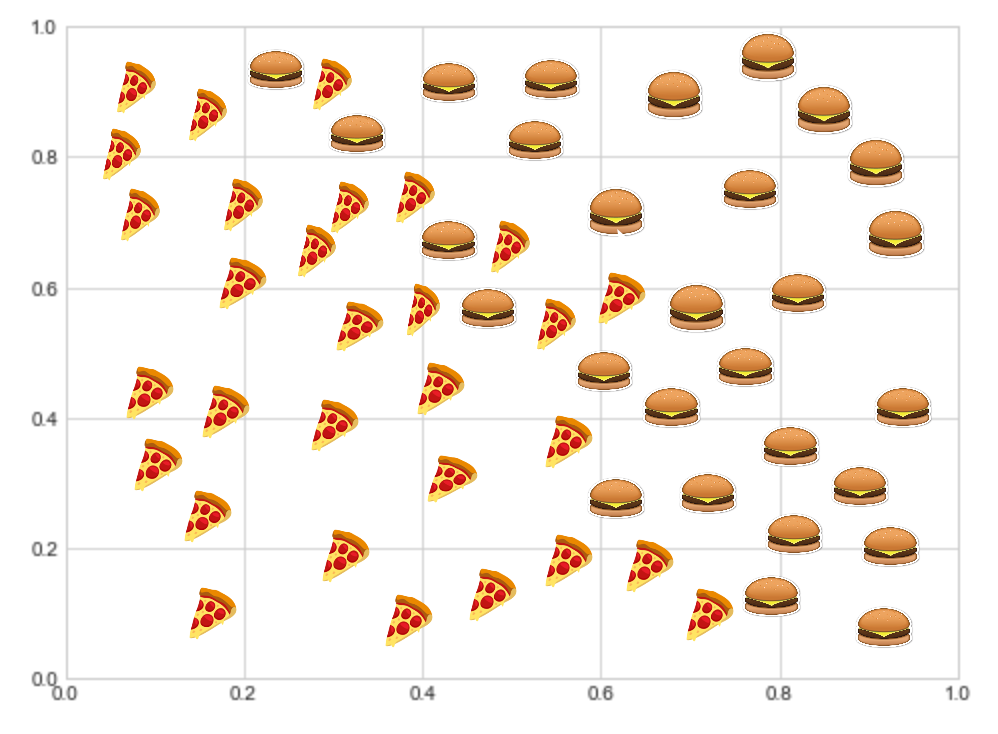
\includegraphics[scale=0.21]{class_1.png}
\end{minipage}
\hfill
\begin{minipage}[t]{0.45\textwidth}
	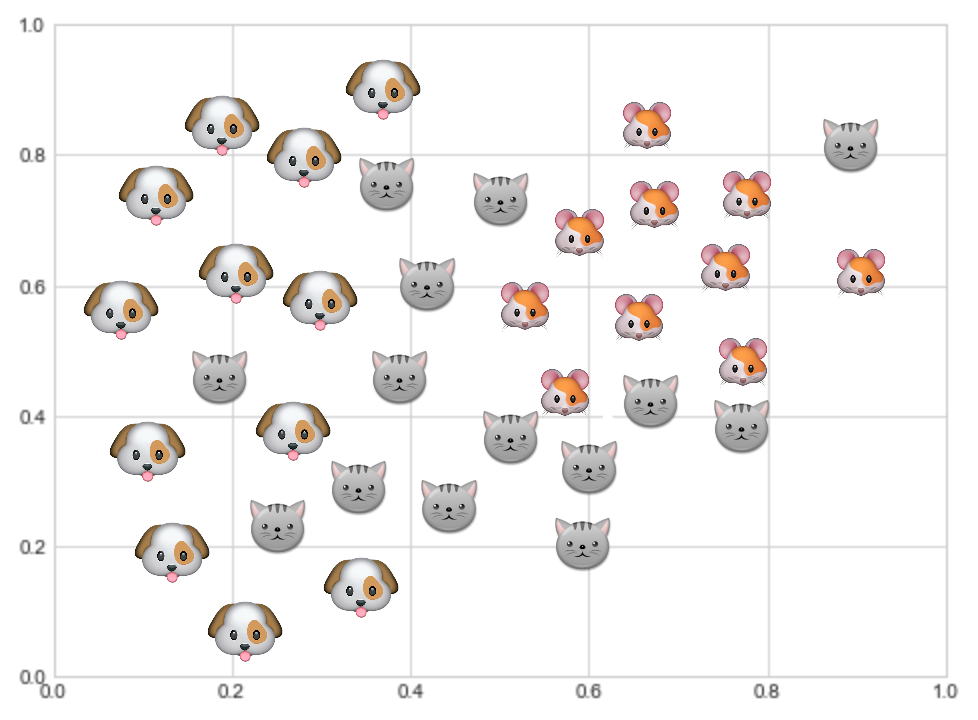
\includegraphics[scale=0.21]{class_2.png}
\end{minipage}

Почему нельзя провести между пиццей и бургерами слишком подробную и извилистую границу? В чём проблема самого правого верхнего котика? Что такое переобучение?  Как понять переобучились ли мы? 
\end{problem}

\begin{solution}
Сначала обсудим бургеры и пиццу.  Первый вариант: провести между ними прямую. Тогда мы в части случаев ошибёмся и признаем некоторые бургеры пиццей, а некоторые пиццы бургерами. Второй вариант: провести извилистую разделительную линию, которая чётко разграничит бургеры и пиццу. Вопрос: какой из этих двух вариантов лучше?
	
\begin{minipage}[t]{0.45\textwidth}
	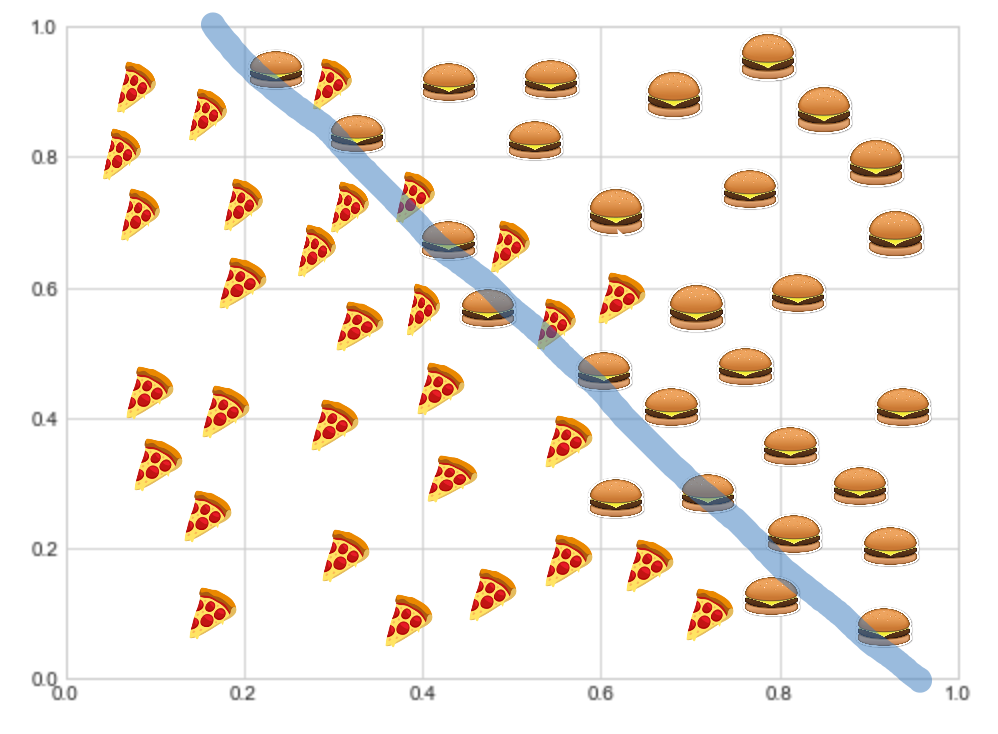
\includegraphics[scale=0.21]{class_1_res1.png}
\end{minipage}
\hfill
\begin{minipage}[t]{0.45\textwidth}
	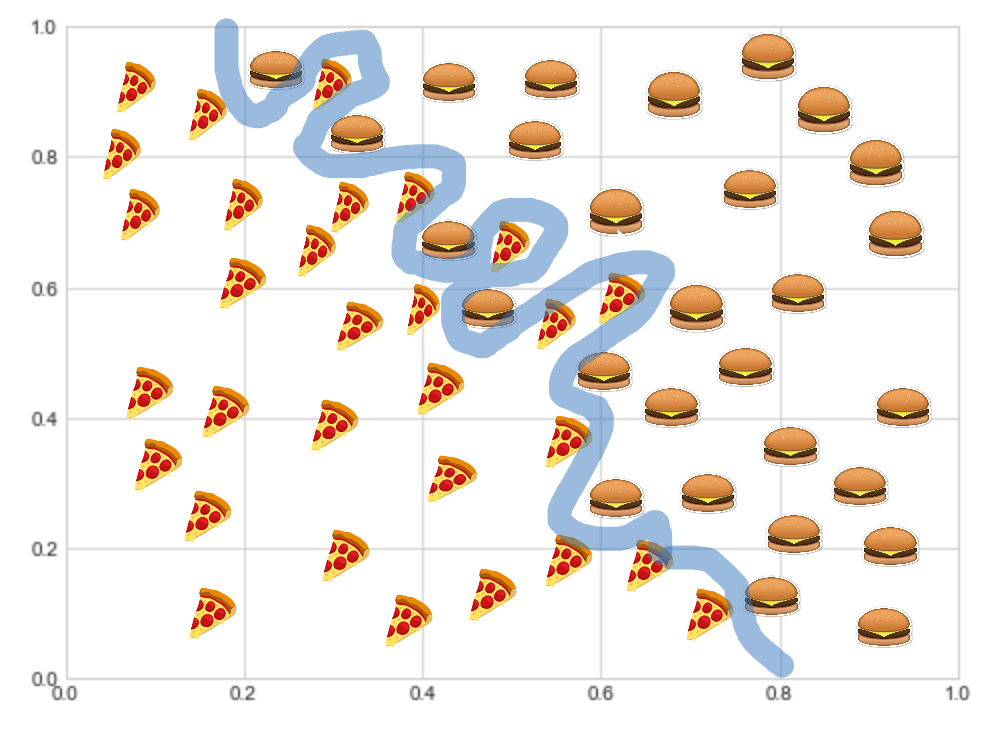
\includegraphics[scale=0.21]{class_1_res2.png}
\end{minipage}
	
Если у нас в выборке оказались все пиццы и бургеры мира, и других быть не может, вторая граница нам подойдёт. Мы подстроимся под все особенности нашей генеральной пицце-бургерной совокупности и будем всегда чётко и безошибочно отличать одно от другого. 

\indef{НО в нашем распряжении обычно находится не вся генеральная совокупность, а лишь какая-то её часть, выборка.} В ней видим не все возможные варианты, и хотим обучить наш классификатор обобщать. Если к нам попадает новая пицца или бургер, классификатор должен адекватно сработать на них. 

Скорее всего, пиццы, проникшие на территорию бургеров, обладают какими-то аномальными особенностями, на детекцию которых затачивать классификатор нет никакого смысла. Если мы попробуем сделать это, мы влезем на территорию бургеров, и на новых объектах, которые оказались обычными бургерами, будем делать ошибки, подумав, что это аномальные пиццы. Из-за этого лучше разграничить бургеры и пиццы простой линией, которая изображена на первой картинке.

\indef{Ещё раз, ещё раз.} Если мы проведём подробную границу, мы заточим классификатор под особенности выборки, вместо того, чтобы научить его отличать пиццу от бургера в общем случае. \indef{Такие ситуации называются переобучением.} И это главная головная боль людей, занимающихся машинным обучением. С переобучением у них идёт вечная борьба. 

Теперь посмотрим на котиков, пёсиков и мышек. Снова мы можем провести границы между ними разными способами.
	
\begin{minipage}[t]{0.45\textwidth}
	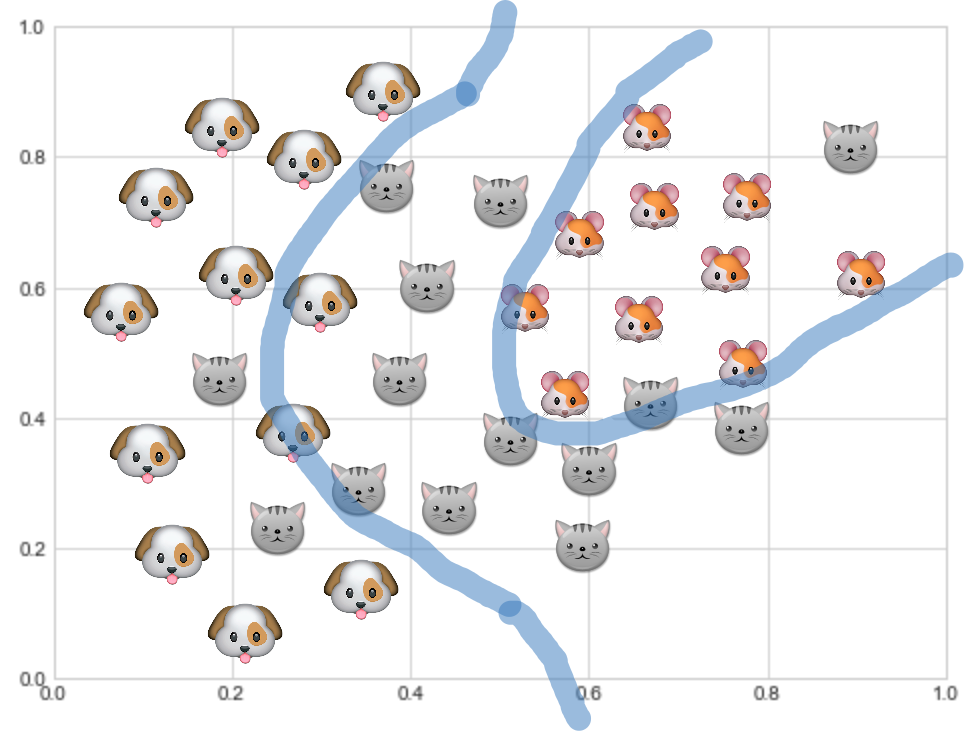
\includegraphics[scale=0.21]{class_2_res1.png}
\end{minipage}
\hfill
\begin{minipage}[t]{0.45\textwidth}
	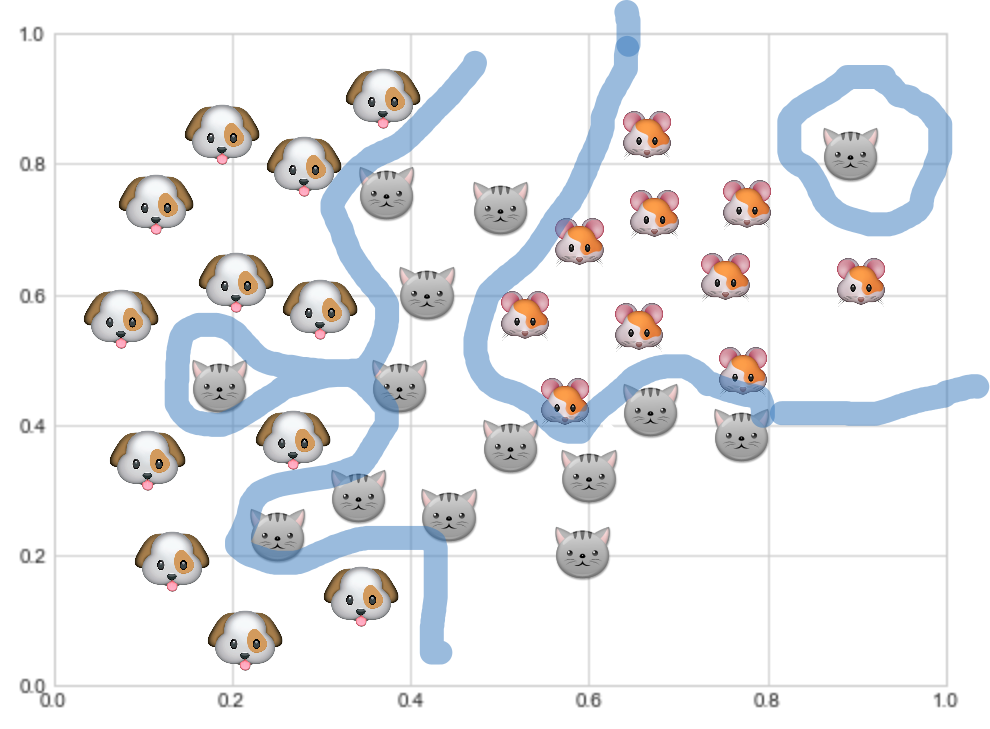
\includegraphics[scale=0.21]{class_2_res2.png}
\end{minipage}

Снова мы можем провести более-менее простую границу и иногда ошибаться. Ну знаете, есть такие собаки мелкие, похожие на кошек. Или даже на мышек\footnote{На самом деле на крыс}. И, если мы будем специфицировать границу под этих собак, мы начнём ошибаться на котах, так как подобные аномалии встречаются редко. 

Основная проблема верхнего котика в том, что он аномальный. Каким-то образом он попал на территорию мышек.  Выделять для него свою зону будет плохой идеей, так как в таком случае мы будем переобучать классификатор под конкретный выброс.

Осталось обсудить главный вопрос: как понять а не переобучились ли мы, когда строили модель, которая должна отделить одни объекты от других? Для этого обычно дробят выборку на две части: \indef{тренировочную и тестовую.} \indef{На тренировочной учат алгоритм} (в данном случае границу между классами), а \indef{на тестовой проверяют насколько хорошо он работает} (сколько и каких ошибок мы допускаем на новых объектах, которые модель раньше не видела)

Если получается, что на обучающей выборке качество высокое, а на тестовой низкое --- мы переобучились и вместо того, чтобы научить модель обобщать закономерности, существующие в данных, обучили его под особенности конкретной выборки.  Если на тестовой выборке качество сравнимо с обучающей, значит мы научились извлекать какие-то реальные закономерности.

Бьюсь об заклад, что для простых линий, качество на тесте для бургеров и мышек будет выше, чем для сложных.  Конечно же, простые границы оказываются хороши не всегда, но тем не менее всегда имеет смысл сначала построить простую модель, а после сравнивать с ней сложные. 
\end{solution}

\begin{problem}
Винни-Пух ищет неправильных пчёл. За долгие годы поиска он скопил довольно большую выборку и оценил на ней три модели: нейросеть, случайный лес и KNN. Он построил на тестовой выборке прогнозы и получил три матрицы ошибок: 

\begin{minipage}[t]{0.3\linewidth}
	\begin{tabular}{|c|c|c|}
		\hline
		& $y=0$  &  $ y = 1$ \\  \hline 
		$\hat y = 0$  &   $80$ &    $20$ \\      \hline 
		$\hat y = 1$ &   $20$ &     $80$ \\      \hline 	
	\end{tabular}
\end{minipage}
\hfill
\begin{minipage}[t]{0.3\linewidth}
	\begin{tabular}{|c|c|c|}
		\hline
		& $y=0$  &  $ y = 1$ \\  \hline 
		$\hat y = 0$  &   $98$ &    $52$ \\      \hline 
		$\hat y = 1$ &   $2$ &     $48$ \\      \hline 		
	\end{tabular}
\end{minipage}
\hfill
\begin{minipage}[t]{0.3\linewidth}
	\begin{tabular}{|c|c|c|}
		\hline
		& $y=0$  &  $ y = 1$ \\  \hline 
		$\hat y = 0$  &   $10000$ &    $90$ \\      \hline 
		$\hat y = 1$ &   $20$ &     $10$ \\      \hline 
	\end{tabular}
\end{minipage}

\begin{enumerate}
	\item[а)]   Найдите для всех трёх моделей долю правильных ответов. Чем плоха эта метрика? 
	\item[б)]   Найдите для всех трёх моделей точность (precision) и полноту (recall)
	\item[в)]   Предположим, что Винни-Пух колектор. Пчела, по его мнению, неправильная, если она не возвращает кредит. Переменная $y$ принимает значение $1$, если пчела вернула кредит  и $0$, если не вернула. ВП хочет научиться прогнозировать платёжеспособность пчелы. Какую из первых двух моделей вы бы выбрали в таком случае? 
	\item[г)]  Предположим, что Винни-Пух врач. Пчела, по его мнению, неправильная, если она умирает от болезни. Он хочет находить таких пчёл и лечить. Переменная $y$ принимает значение $1$, если пчела больна больной болезнью с болью и $0$, если она здорова. ВП хочет спрогнозировать нужно ли пчеле пройти обследование. Какую из первых двух моделей вы б выбрали в этом случае? 
	\item[д)] Найдите для всех трёх моделей f1-меру. 
\end{enumerate}
\end{problem}

\begin{solution}
	\begin{enumerate}
		\item[а)] 	Ежели мы совершаем ошибку, то мы делаем это, когда прогнозируем $\hat y = 1$ там, где реально должно быть $y = 0$, либо наоборот, прогнозируя $\hat y = 0$ там, где реально должно быть $y=1$.  В остальных случаях ошибки нет.  Наша классная табличка выглядит следующим образом: 
		
	\begin{center}
		\begin{tabular}{|c|c|c|}
		\hline
		& $y=0$  &  $ y = 1$ \\  \hline 
		$\hat y = 0$  &   $TN$ &    $FN$ \\      \hline 
		$\hat y = 1$ &   $FP$ &     $TP$ \\      \hline 
		\end{tabular}
	\end{center}
		
		В ней $TP$ --- True Positive, то есть мы спрогнозировали $1$ и не ошиблись, $FP$ --- False Positive, то есть мы спрогнозировали $1$ и ошиблись. По аналогии с $FN$ --- False Negative и  $TN$ --- True Negative. Долю правильных ответов можно посчитать как 
		
		\[
		Accuracy = \frac{TP + TN}{TP + TN + FP + FN}.
		\]
		
		Давайте проделаем эту несложную процедуру для вердиктов всех трёх алгоритмов, описанных выше. 
		
		\begin{equation} 
		\begin{aligned}
		&Accuracy_1 = \frac{80 + 80}{80 + 80 + 20 + 20} = 0.8   \\ 
		&Accuracy_2 = \frac{48 + 98}{48 + 98 + 2 + 52} = 0.73  \\ 
		&Accuracy_3 = \frac{10 + 10000}{10 + 10000 + 20 + 90} = 0.98  \\ 
		\end{aligned}
		\end{equation} 
		
		У этой метрики есть как минимум две существенные проблемы. 
		
		Первая проблема связана с несбалансированными выборками. Именно такая ситуация наблюдается в третьей табличке. Нулевой класс заметно перетягивает на себя выборку. Выходит, что если мы просто-напросто спрогнозируем, что все объекты в выборке нулевые, мы получим табличку 
		
		\begin{center}
			\begin{tabular}{|c|c|c|}
					\hline
		& $y=0$  &  $ y = 1$ \\  \hline 
		$\hat y = 0$  &   $10020$ &    $100$ \\      \hline 
		$\hat y = 1$ &   $0$ &     $0$ \\      \hline 
			\end{tabular}
		\end{center}
		
		и $Accuracy = 0.99$. Наша модель показала более низкое качество, чем простое угадывание. Выходит, что наша модель с точки зрения этой метрики абсолютно бесполезна. 
		
		Чтобы «бороться» с этой проблемой, используется следующий факт. Пусть $q_0$ — доля объектов самого крупного класса, тогда доля правильных ответов для разумных алгоритмов $accuracy \in [q_0; 1]$, а не $[0.5; 1]$, как это можно было бы ожидать. Поэтому, если получается высокий процент правильных ответов, это может быть связано не с тем, что построен хороший классификатор, а с тем, что какого-то класса сильно больше, чем остальных.
		
		Вторая проблема с долей верных ответов состоит в том, что она никак не учитывает разные цены разных типов ошибок.
		
		Например, представим себе линейное небо, которое бороздят вражеские самолёты. Мы стоим на земле, у нас есть пушка и снаряды. Сбивать вражеские самолёты можно руководствуясь двумя разными стратегиями: 
		
		\textbf{Путь первый:}  стрелять по всему небу, куда только можно попасть. В таком случае точность наших выстрелов будет низкой, но зато мы собьём все самолёты, то есть добьёмся высокой полноты. Такая стратегия на картинке прорисована красными лазерными выстрелами из пушки.
		
		\textbf{Путь второй:} стрелять поточнее, но реже. Тогда мы будем сбивать самолёты точно, потратим мало снарядов вхолостую, но собьём не все самолёты. Такая стратегия на картинке прорисована зелёными выстрелами из пушки. 
		
		\begin{center}
			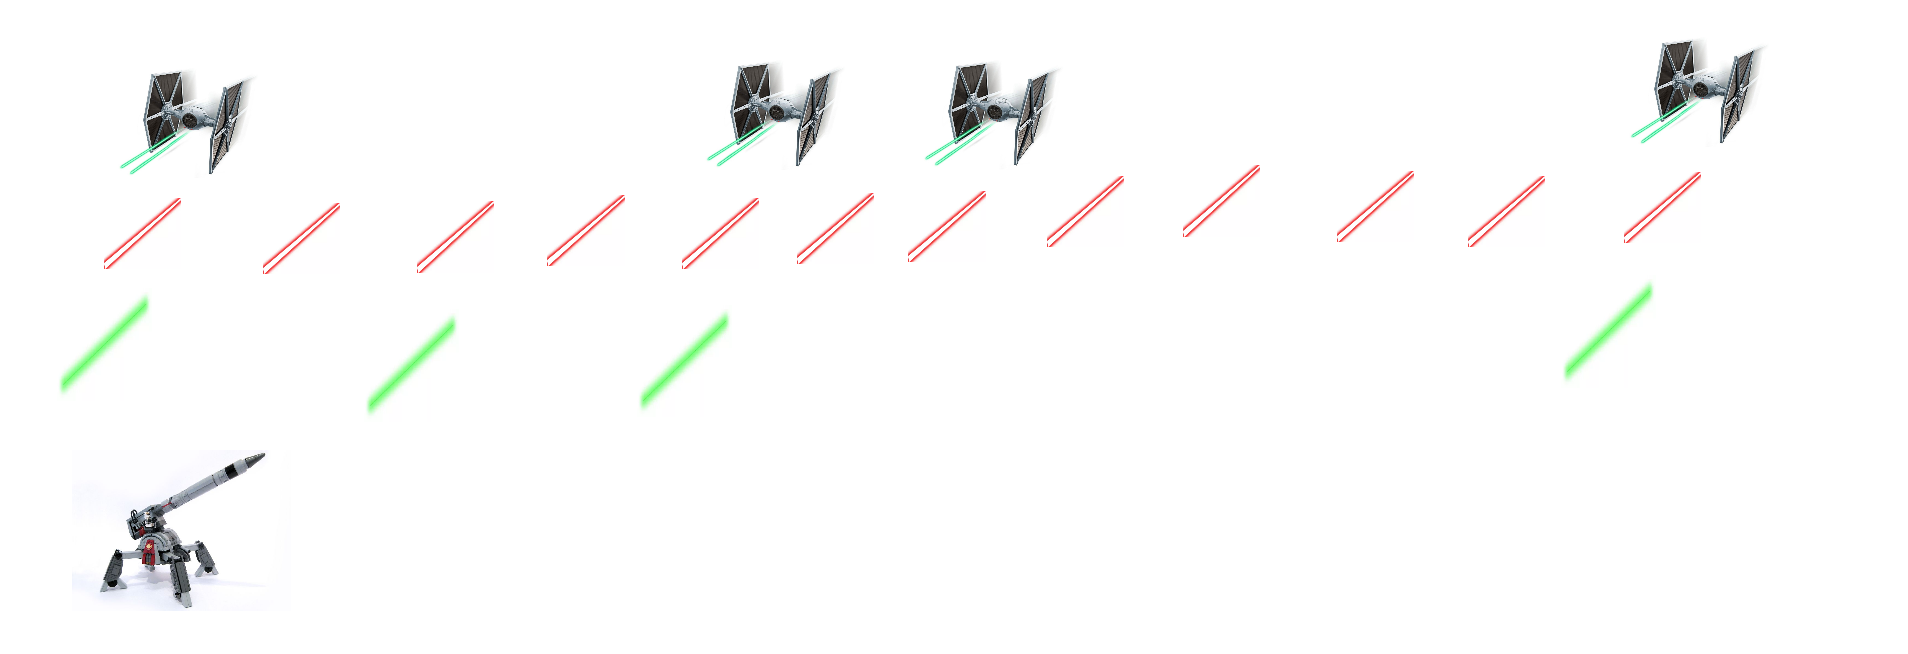
\includegraphics[width=.79\paperwidth]{fly.png}
		\end{center}
		
		Для разных задач бывают характерны разные стратегии. Если вернуться к нашей исходной таблице ошибок, то за точность классификатора будет отвечать первая строка
		
		\[ 
		Precision = \frac{TP}{TP + FP}.
		\]
		
		За полноту будет отвечать первый столбец
		
		\[Recall = \frac{TP}{TP + FN}.\]
		
		Посмотрим ещё один пример: если мы решаем задачу крединтого скоринга, выдаём пчёлам кредит, нам нужно получить деньги назад с процентом, иначе мы разоримся. Нам нужна модель, которая будет точно определять надёжного заёмщика. В этой ситуации для нас неважно покрыть все вражеские истребители снарядами (выдать кредиты каждой надёжной пчеле), для нас важно сделать это точно. Поэтому основное внимание мы уделяем ошибке $FP$, и ищем точный алгоритм. 
		
		Если мы пытаемся найти больных больной болезнью с болью и отправить их делать дополнительные анализы, для нас страшнее $FN$ ошибка. Если мы отправим лишнего человека на анализы, ничего страшного с ним не произойдёт. Если мы забудем проверить больного, он умрёт. Тут лучше добиться высокой полноты, при небольшой точности. 
		
		В разных ситуациях ошибки имеют разные цены. $Accuracy$ не видит этого, поэтому на практике обычно используют $Precision$ и $Recall$. 
		
		\item[б)]  Найдём их для наших трёх моделей: 
		
		\begin{equation} 
		\begin{aligned}
		&Precision_1 =  0.8   \qquad &Recall_1 = 0.8 \\ 
		&Precision_2 = 0.96  \qquad &Recall_2 = 0.48 \\ 
		&Precision_3 = 0.33  \qquad &Recall_3 = 0.1  \\
		\end{aligned}
		\end{equation} 
		
		Вторая модель является очень точной, но в ущерб полноте. Третья модель очень плохая. Эти две метрики, в отличие от $Accuracy$, позволили заметить этот факт. 
		
		\item[в)] При использовании первой модели кредит будет выдан 100 клиентам, 80 из которых его вернут. Во второй модели, более консервативной, кредит был выдан только 50 клиентам, причем вернули его в 48 случаях. 
		
		Выше мы обсудили, что бизнес-специфика задачи диктует нам необходимость взять модель, где побольше точность.
		
		\item[г)]  Выше мы обсудили, что нам нужна модель, где побольше полнота.
		
		\item[д)]  Чем выше точность и полнота, тем лучше. Однако в реальном мире невозможно добиться того, чтобы оба показателя были очень большими. Между ними приходится искать какой-то баланс. Чтобы видеть его, хочется объединить точность и полноту в какую-то общую метрику. Такой метрикой является \indef{f-мера.} Посчитать её можно по формуле: 
		
		$$
		f = 2 \cdot \frac{precision \cdot recall}{precision + recall}.
		$$
		
		Сделаем это для наших моделей: 
		
		\begin{equation} 
		\begin{aligned}
		&f_1 =  2 \cdot \frac{0.8 \cdot 0.8}{0.8 + 0.8} = 0.8 \\
		&f_2 =  2 \cdot \frac{0.96 \cdot 0.48}{0.96 + 0.48} = 0.64 \\
		&f_3 =  2 \cdot \frac{0.33 \cdot 0.1}{0.33 + 0.1} = 0.15 \\
		\end{aligned}
		\end{equation} 
		
		Видим, что первая модель оказывается в терминах f-меры самой хорошей. 
		
		F-мера --- это гармоническое среднее между точностью и полнотой. Среднее гармоническое обладает важным свойством --- оно близко к нулю, если хотя бы один из аргументов близок к нулю. Именно поэтому оно является более предпочтительным, чем среднее арифметическое (если алгоритм будет относить все объекты к положительному классу, то он будет иметь $recall = 1$ и $precision << 1$, а их среднее арифметическое будет больше $0.5$, что недопустимо).
		
		Можно попробовать нарисовать эту метрику в координах точность-полнота и получить вот такие кривые: 

\begin{center}
    \begin{tikzpicture}[/pgfplots/width=10cm, /pgfplots/height=10cm]
        \begin{axis}[% Axis labels
                     ymin=0,ymax=1,xmin=0,xmax=1,
        			 % Axis labels
            		 xlabel=Recall,
            		 ylabel=Precision,
             		 xlabel shift={-2pt},
            		 ylabel shift={-3pt},
             		 % General appearance
    		         font=\small,
    		         axis equal image=true,
    		         enlargelimits=false,
    		         clip=false,
    		         % Grids 
            	     grid style=dotted, grid=both,
                     major grid style={white!65!black},
            		 minor grid style={white!85!black},
    		 		 xtick={0,0.1,...,1.1},
            		 ytick={0,0.1,...,1.1},
             		 minor xtick={0,0.02,...,1},
    		         minor ytick={0,0.02,...,1},
            		 % Legend
            		 legend style={at={(0,0)},
                     		       anchor=south west}]
            
        % Iso-f curves
        \foreach \f in {0.1,0.2,...,0.9}{%
           \addplot[blue,line width=0.2pt,domain=(\f/(2-\f)):1,samples=200,forget plot]{(\f*x)/(2*x-\f)};
        }
        \end{axis}
    \end{tikzpicture}
\end{center}

Вдоль каждой кривой f-мера постоянна. Например, для самой нижней кривой, а-мера равна $0.1$. Чем правее по ней мы сдвигаемся тем меньше точности и тем больше полнота. Прирост полноты вдоль кривой компенсирует упадок точности и мы остаемся на том же самом уровне f-меры. 

Если вы когда-нибудь изучали микроэкономику, то вам в голову должна была прийти аналогия с кривыми безразличия. Точность и полнота в данной ситуации это товары. f-мера --- полезность от их потребления. Вдоль каждой кривой безразличия  мы замещаем один товар другим и остаемся на том же уровне полезности. 

Можно попробовать дать больший вес точности или полноте, если от нас требует этого задача и немного вытянуть кривые безразличия в сторону полноты или точности: 

	$$
	f = (\beta^2 + 1) \cdot \frac{precision \cdot recall}{\beta^2 \cdot precision + recall}.
	$$

Если $\beta > 1$ приоритет отдаётся полноте, если $0 < \beta < 1$, то точности. Например, если $\beta = 2$, для нас более важна полнота.  Если $\beta = 0.5$, более важна точность. 
\end{enumerate}
\end{solution}


\begin{problem} 
Бандерлог из Лога\footnote{деревня в Кадуйском районе Вологодской области} ведёт блог, любит считать логарифмы и оценивать модели\footnote{Читай больше про приключения Бандерлога тут: \url{https://github.com/bdemeshev/mlearn_pro}}. С помощью нового алгоритма Бандерлог решил задачу классификации по трём наблюдениям и получил $\hat p_i = \hat P(y_i = 1|x_i)$.

\begin{center}
	\begin{tabular}{c|c}
		$y_i$ & $\hat p_i$ \\
		\hline
		$1$  & $0.7$ \\
		$0$ & $0.2$ \\
		$0$ & $0.3$ \\
		$1$ & $0.25$ \\
		$0$ & $0.1$ \\
	\end{tabular}
\end{center}

\begin{enumerate}
	\item[a)] Найдите ROC AUC.
	\item[б)] Постройте ROC-кривую.
	\item[в)] Постройте PR-кривую (кривая точность-полнота).
	\item[г)] Найдите площадь под PR-кривой.
	\item[д)] Как по-английски будет «бревно»?
\end{enumerate}
\end{problem} 

\begin{solution}
В предыдущей задаче мы немного обсудили метрики классификации. Когда мы на практике оцениваем модель, она, чаще всего, выплёвывает в нас не принадлежность объекта к классу в явном виде, а вероятности того, что наши объекты --- единички. 
		
Например, давайте думать в терминах оттока клиентов. Пусть наш сервис привлёк каких-то ребят в постоянные пользователи. Если они начнут унывать, им захочется свалить. Это называется оттоком. Давайте предположим, что модель выдаёт нам вероятность того, что человек решил приуныть. Если мы сможем понимать кто собрался приуныть, будем одаривать их ништяками и тогда они будут оставаться нашими клиентами. 
	
Как понять, кто собирается приуныть, если модель выплёвывает на нас вероятности? Давайте выберем порог и будем считать, что все, у кого вероятность уныния $\ge 0.5$  относятся к классу $1$. Есть вероятность, что они решат свалить. Их и будем одаривать ништяками. В нем случае получатся прогнозы: $1,0,0,0,0$. Если взять порог $0.3$, получим прогнозы $1,0,1,0,0$. 

Как выбрать порог, кого одаривать ништяками? Если у нас большой бюджет, можно попробовать поставить низкий порог, чтобы добиться большой полноты. Если маленький бюджет, то давайте поставим порог так, чтобы борьба с унынием была поточнее. Выбор порога зависит от специфики бизнеса и от того, что от нас хотят. 
	
Видно, что точность и полнота зависят от выбора порога. А хотелось бы, чтобы та метрика, по которой мы выбираем модель, от порога не зависела. \indef{Так рождаются идеи о метриках $roc\_auc$ и $pr\_auc$.} 

\begin{enumerate}	
    \item[а)]  Представим себе два объекта: приунывший и нормальный. Представим себе, что модель предсказала нам вероятность уныния для первого объекта $\hat p_1$ и для второго $\hat p_2$.
	
	\begin{equation} 
	\begin{aligned}
	&y = 1   \qquad &\hat P(y = 1) = \hat p_1\\ 
	&y = 0  \qquad & \hat P(y = 1) = \hat p_2\\ 
	\end{aligned}
	\end{equation} 
	
	Если у нас хорошая модель, то явно $\hat p_1 > \hat p_2$. Иначе модель всё путает и говорит, что неунывающие приуныли. Давайте посмотрим как часто на нашей выборке такая путаница происходит и \indef{рассмотрим все возможные пары нулей и единичек.} Всего будет шесть пар. 
	
	\begin{equation} 
	\begin{aligned}
	& 0.7 > 0.2 \qquad & ok \\
	& 0.7 > 0.3 \qquad & ok \\
	& 0.7 > 0.1 \qquad & ok \\
	& 0.25 > 0.2 \qquad & ok \\ 
	& 0.25 < 0.3 \qquad & not \mbox{ } ok \\
	& 0.25 > 0.1 \qquad & ok \\
	\end{aligned}
	\end{equation} 

    Отдельно обращаю ваше внимание, что не надо смотреть на пары из только нулей и только единичек. На самостоятельной работе часто люди смотрят на них тоже. Это ошибка.

	Видим, что модель ошиблась в упорядочивании один раз. $roc\_auc$ --- это доля пар, где модель оказалась права. В нашем случае это $\frac{5}{6}$. $roc\_auc$ принимает значения от $0.5$ до $1$, если её значения близки к $0.5$, наш алгоритм ничем не лучше монетки, потому что он упорядочивает пары из унывших и нормальных случайно. 

	Такая метрика позволяет не привязываться к конкретному значению порога и видеть насколько классно у модели выходит упорядочивать пары объектов. 

	\item[б)]  Величина, которую мы посчитали выше является площадью под roc-кривой (roc = receiver operating characteristic, иногда говорят «кривая ошибок»), с помощью которой часто визуализируют качество работы алгоритма.  Когда говорять про roc-auc имется в виду area under the curve\footnote{\href{https://dyakonov.org/2017/07/28/}{В блоге Дьяконова} есть ещё задачки на ROC-AUC и объяснение что это за кривая, прочтите на досуге}. 

	Чтобы нарисовать ROC-кривую, надо взять единичный квадрат на координатной плоскости, разбить его на m равных частей горизонтальными линиями и на $n$ – вертикальными, где $m$ – число $1$ среди правильных меток теста (в нашем примере $m=2$), $n$ – число нулей ($n=3$). В результате квадрат разбивается сеткой на $m \times n$ блоков.
	
	\indef{Отсортируем нашу табличку по значению вероятности, которую предсказала модель} (в самостоятельной это тоже часто забывают сделать, обратите на это внимание).
	
	\begin{center}
		\begin{tabular}{c|c}
			$y_i$ & $\hat p_i$ \\
			\hline
			$1$  & $0.7$ \\
			$0$ & $0.3$ \\
			$1$ & $0.25$ \\
			$0$ & $0.2$ \\
			$0$ & $0.1$ \\
		\end{tabular}
	\end{center}
	
	Теперь будем просматривать строки сверху вниз и прорисовывать на сетке линии, переходя их одного узла в другой. Стартуем из точки $(0, 0)$. Если значение метки класса в просматриваемой строке $1$, то делаем шаг вверх; если $0$, то делаем шаг вправо. Ясно, что в итоге мы попадём в точку $(1, 1)$, т.к. сделаем в сумме $m$ шагов вверх и $n$ шагов вправо.
		
\begin{center}
    \begin{tikzpicture}[line cap=round,line join=round,x=1.5cm,y=1.5cm]
    
    \draw [->,line width=1.pt] (-0.3,0) -- (3.5,0);
    \draw [->,line width=1.pt] (0,-0.3) -- (0,3.5);
    
    \fill[line width=2.pt,color=litebrown,fill=litebrown,fill opacity=0.10000000149011612] (0,0) -- (0,1.5) -- (1,1.5) -- (1,3) -- (2,3) -- (3,3) -- (3,0) -- cycle;
    
    \draw [line width=1.5pt,color=litebrown] ((0,0) -- (0,1.5) -- (1,1.5) -- (1,3) -- (2,3) -- (3,3) -- (3,0) -- cycle;
    
    \draw [fill=blue] (0,0) circle (3pt);
    \draw [fill=blue] (0,1.5) circle (3pt);
    \draw [fill=blue] (1,1.5) circle (3pt);
    \draw [fill=blue] (1,3) circle (3pt);
    \draw [fill=blue] (2,3) circle (3pt);
    \draw [fill=blue] (3,3) circle (3pt);
    
    \draw [line width=1.pt, dotted] (0,3) -- (1,3);
    \draw [line width=1.pt, dotted] (1,0) -- (1,1.5);
    \draw [line width=1.pt, dotted] (1,1.5) -- (3,1.5);
    \draw [line width=1.pt, dotted] (2,0) -- (2,3);
    
    \draw (3, 0) node[anchor=north] {$1$};
    \draw (0, 3) node[anchor=east] {$1$};
    \end{tikzpicture}
\end{center}
    
    \indef{Важный момент:} если у нескольких объектов значения оценок равны, то мы делаем шаг в точку, которая на $a$ блоков выше и $b$ блоков правее, где $a$ --- число единиц в группе объектов с одним значением метки, $b$ --- число нулей в ней. Непонятно? Проработайте задачку из \href{ https://dyakonov.org/2017/07/28/}{блога Дьяконова.} Она там как раз такая. 
  
	Сетка разбила квадрат на  $m \times n$ блоков. Ровно столько же пар вида (объект класса $1$, объект класса $0$), составленных из объектов тестовой выборки. Каждый закрашенный блок соответствует паре (объект класса $1$, объект класса $0$), для которой наш алгоритм правильно предсказал порядок (объект класса $1$ получил оценку выше, чем объект класса $0$), не закрашенный блок --– паре, на которой ошибся.
	
	Можно объяснять построение кривой немного иначе, в терминах $FPR$ --- False Positive Rate и $TPR$ --- True Positive Rate. Но любой нормальный человек сразу же забывет эти стрёмные буквы. Тем не менее, по оси $x$ на нешей картинке отложена именно $FPR$, а по оси $y$ отложена $TPR$: 
	
\begin{center}
    \begin{tikzpicture}[line cap=round,line join=round,x=1.5cm,y=1.5cm]
    
    \draw [->,line width=1.pt] (-0.3,0) -- (3.5,0);
    \draw [->,line width=1.pt] (0,-0.3) -- (0,3.5);
    
    \fill[line width=2.pt,color=litebrown,fill=litebrown,fill opacity=0.10000000149011612] (0,0) -- (0,1.5) -- (1,1.5) -- (1,3) -- (2,3) -- (3,3) -- (3,0) -- cycle;
    
    \draw [line width=1.5pt,color=litebrown] ((0,0) -- (0,1.5) -- (1,1.5) -- (1,3) -- (2,3) -- (3,3) -- (3,0) -- cycle;
    
    \draw [fill=blue] (1,1.5) circle (3pt);
    
    \draw [line width=1.pt, dotted] (0,3) -- (1,3);
    \draw [line width=1.pt, dotted] (1,0) -- (1,1.5);
    \draw [line width=1.pt, dotted] (1,1.5) -- (3,1.5);
    \draw [line width=1.pt, dotted] (2,0) -- (2,3);
    
    \draw (3, 0) node[anchor=north] {$1$};
    \draw (0, 3) node[anchor=east] {$1$};

    \draw (3.5, -0.1) node[anchor=north] {$FPR$};
    \draw (-0.1, 3.5) node[anchor=east] {$TPR$};
    \end{tikzpicture}
\end{center}

	Выбору порога соответствует выбор точки на $ROC$-кривой. Например, на картинке выше нарисована точка, которая соответствует порогу между $0.3$ и $0.25$. Например,всё, что больше $0.27$ мы объявляем единицей. Если двигать порог в рамках указанного выше диапазона, ничего меняться не будет.
	
	Мы видим, что $FPR = \frac{1}{3}$ --- это процент точек класса 0, которые неверно классифицированы нашим алгоритмом, а $TPR = 0.5$ --- процент точек класса 1, которые верно классифицированы нашим алгоритмом. Кстати говоря, $TPR$ и полнота, $recall$, это одно и то же.
	
    Метрика классная и интуитивно понятная, но страдает большой проблемой: она чувствительна к дисбалансу в классах. Также как и $Accuracy$.
    
    Например, пусть у нас есть $100 000$ пчёл и $100$ из них неправильные. Если алгоритм идеально понимает какие $100$ пчёл неправильные, мы получаем $TPR = 1$ и $FPR = 0$. 
    
    Посмотрим теперь на плохой алгоритм, который находит $95$ неправильных пчёл из $100$ и объявляет $50 000$ правильных пчёл плохими. Для такого алгоритма получится $TPR = 0.95$, а $FPR = 0.05$. Это довольно близко к идеальному алгоритму, хотя при этом точность алгоритма оставляет желать лучшего. 
    
    \indef{Если положительный класс существенно меньше по размеру, $roc\_auc$ может давать неадекватную оценку качества алгоритма.} Вылечить такой недостаток позволяет другая метрика, $pr\_auc$ (precision-recall area under curve). 

	\item[в)] Давайте по оси $x$ откладывать полноту, а по оси $y$ точность. Будем по очереди перебирать разные пороги и считать для них точность и полноту. Нанесём на картинку все полученные точки и соединим их. Это и будет \indef{$precision-recall$ кривая.}
	
	Например, если мы возьмём порог $ \ge 0.1$, тогда все объекты будут принадлежать к классу $1$ точность составит $\frac{2}{5}$, а полнота $1$.  Если мы возьмём порог $\ge 0.2$, тогда один объект будет нулевым, а остальные четыре единичными.  Точность составит $\frac{2}{4}$, а полнота $1$.  По аналогии получим точность и полноту при порогах $\ge 0.25$, $\ge 0.3$ и $\ge 0.7$. 
	
	\begin{center}
		\begin{tabular}{c|c|c}
			порог &точность  & полнота\\
			\hline
			$0.1$ & $\frac{2}{5}$ & $1$ \\
			$0.2$ & $\frac{2}{4}$ & $1$ \\
			$0.25$ & $\frac{2}{3}$ & $1$ \\
			$0.3$ & $\frac{1}{2}$ & $\frac{1}{2}$ \\
			$0.7$ & $1$& $\frac{1}{2}$ \\
			$0.8$ & $0$ & $0$ \\
		\end{tabular}
	\end{center}
	
	Строим кривую! 

\begin{center}
    \begin{tikzpicture}[line cap=round,line join=round,x=5cm,y=5cm]
    
    \draw [->,line width=1.pt] (-0.1,0) -- (1.1,0);
    \draw [->,line width=1.pt] (0,-0.1) -- (0,1.1);
    
    \fill[line width=2.pt,color=litebrown,fill=litebrown,fill opacity=0.1] (0,0) -- (0.5,1) -- (0.5,0.5) -- (1,0.66) -- (1,0.5) -- (1,0.4) -- (1,0) -- cycle;
    
    \draw [line width=1.5pt,color=litebrown] (0,0) -- (0.5,1) -- (0.5,0.5) -- (1,0.66) -- (1,0.5) -- (1,0.4) -- (1,0) -- cycle;
    
    \draw [fill=blue] (0,0) circle (3pt);
    \draw [fill=blue] (0.5,1) circle (3pt);
    \draw [fill=blue] (0.5,0.5) circle (3pt);
    \draw [fill=blue] (1,0.66) circle (3pt);
    \draw [fill=blue] (1,0.5) circle (3pt);
    \draw [fill=blue] (1,0.4) circle (3pt);
    
    \draw [line width=1.pt, dotted] (0.5,0.5) -- (0.5,0);
    \draw [line width=1.pt, dotted] (0,0.5) -- (1,0.5);
    \draw [line width=1.pt, dotted] (0,0.4) -- (1,0.4);
    \draw [line width=1.pt, dotted] (0,1) -- (0.5,1);
    \draw [line width=1.pt, dotted] (0,0.66) -- (1,0.66);
    
    \draw (0.5, 0) node[anchor=north] {$0.5$};
    \draw (0, 0.5) node[anchor=east] {$0.5$};
    \draw (0, 0.4) node[anchor=east] {$0.4$};
    \draw (0, 1) node[anchor=east] {$1$};
    \draw (0, 0.66) node[anchor=east] {$0.66$};
    \draw (1, 0) node[anchor=north] {$1$};

    \draw (1.2, 0) node[anchor=north] {$recall$};
    \draw (0, 1.12) node[anchor=east] {$precision$};
    \end{tikzpicture}
\end{center}

	PR- кривая всегда начинается из точки $(0,0)$ и заканчивается в точке $(1,r)$, где $r$ --- это доля объектов первого класса в выборке. Иногда для красоты кривую рисуют из точки $(0,1)$. Например, так делает sklearn.
	
	В случае идеального классификатора, то есть если существует такой порог, что и точность, и полнота равны $100\%$, кривая будет проходить через точку $(1, 1)$. Таким образом, чем ближе кривая пройдет к этой точке, тем лучше оценки. Площадь под этой кривой может быть хорошей мерой качества оценок принадлежности к классу $1$. Такая метрика называется pr-auc, или площадь под PR-кривой.

	\item[г)] Посчитав площадь под кривой получим pr-auc.  Будем делать это, считая площади треугольников и прямоугольников. 
	
	\[
	0.5 \cdot 1\cdot 0.5 + 0.5 \cdot 0.5 \cdot (0.66 - 0.5) + 0.5^2 = 0.25 + 0.04 + 0.25 = 0.54
	\]

	Эта метрика подобно roc-auc не зависит от выбора порога и отражает способность модели правильно упорядочивать пары, но немножечко в другом плане. Эта метрика строится в осях точность и полнота. Из-за этого она нечувствительна к дисбалансу в выборке. В примере с пчёлами мы получаем, что $recall = 0.95$, а $precision = \frac{95}{50095}$, и видим, что алгоритм не очень удачный. 
	
	Кстати говоря, если снова обратиться к микроэкономике, можно провести аналогию между pr-кривой и допустимым множеством товаров. Самая классное сочетания precision и recall, доступное нам, лежит на самой высокой f-кривой (кривой безразличия), касающейся precision-recall кривой. 
	
	\begin{center}
	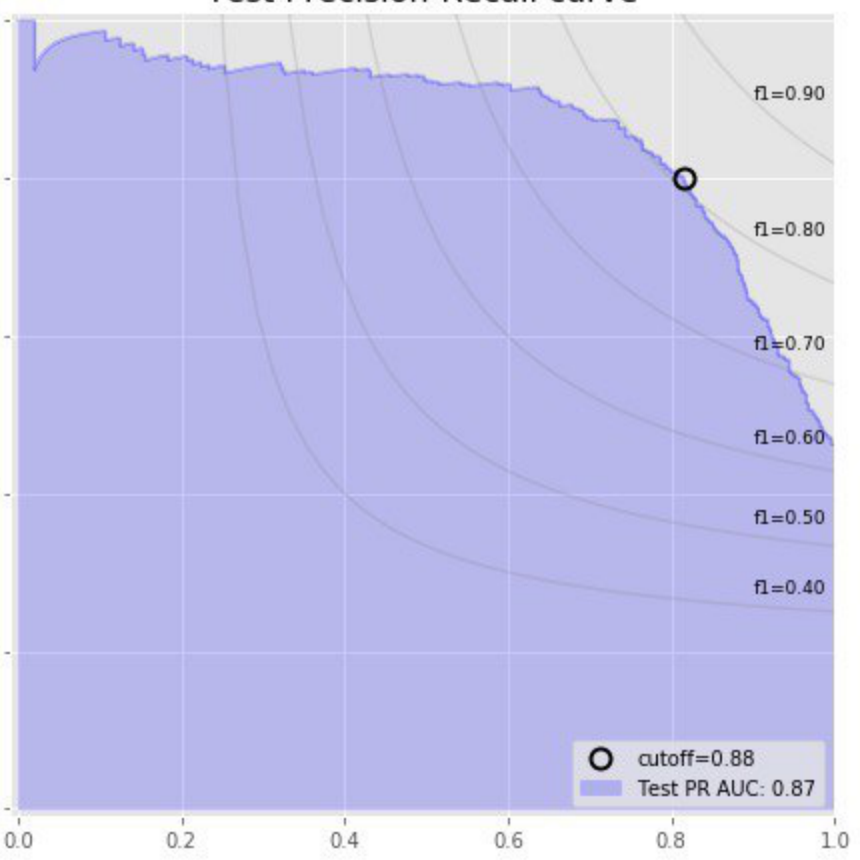
\includegraphics[scale=0.6]{pr_rec.png}
	\end{center}
	
	\todo[inline]{Заменить картинку на нормальную}
	
	\item[д)]  log 
	
	\end{enumerate}
\end{solution}


\section*{Ещё задачи!}

Тут лежит ещё несколько задач для самостоятельного решения. Возможно, похожие будут в самостоятельной работе... 


\begin{problem}
Бандерлог начинает все определения со слов «это доля правильных ответов»:
\begin{enumerate}
	\item[а)] accuracy — это доля правильных ответов\ldots
	\item[б)] точность (precision) — это доля правильных ответов\ldots
	\item[в)] полнота (recall) — это доля правильных ответов\ldots
	\item[г)] TPR — это доля правильных ответов\ldots
\end{enumerate}

Закончите определения Бандерлога так, чтобы они были, хм, правильными.
\end{problem} 

\begin{problem}
    Бандерлог обучил модель для классификации и получил вектор предсказанных вероятностей принадлежностей к классу $1$. 
    
    \begin{center}
    	\begin{tabular}{c|c}
    		$y_i$ & $b_i$ \\
    		\hline
    		$1$  & $0.9$ \\
    		$0$ & $0.1$ \\
    		$0$ & $0.75$ \\
    		$1$ & $0.56$ \\
    		$1$ & $0.2$ \\
    		$0$ & $0.37$ \\
    		$0$ & $0.25$ \\		
    	\end{tabular}
    \end{center}
    
    \begin{enumerate}
    	\item[а)]  Бинаризуйте ответ по порогу $t$ и посчитайте точность и полноту для $t = 0.3$ и для  $t = 0.8$.
    	\item[б)]  Какой порог вы бы выбрали? 
    	\item[в)]  Постройте ROC-кривую и найдите площадь под ней. 
    \end{enumerate}
\end{problem} 

\begin{solution}
	\begin{enumerate}
		\item[а)]  Построим в нашей табличке две колонки с прогнозами. Для удобства. 
		
		\begin{center}
			\begin{tabular}{c|c|c|c}
				$y_i$ & $b_i$ & $t=0.3$  & $t=0.8$\\
				\hline
				$1$  & $0.9$ & $1$ & $1$ \\
				$0$ & $0.1$ & $0$ & $0$\\
				$0$ & $0.75$ & $1$ & $0$\\
				$1$ & $0.56$ & $1$ & $0$\\
				$1$ & $0.2$ & $0$ & $0$ \\
				$0$ & $0.37$ & $1$ & $0$\\
				$0$ & $0.25$ & $0$ & $0$ \\		
			\end{tabular}
		\end{center}
		
		Построим для обоих порогов матрицы ошибок. Слева матрица, соответствующая порогу $0.3$, справа матрица, соответствующая порогу $0.8$.
		
		\begin{minipage}[t]{0.45\textwidth}
			\begin{tabular}{|c|c|c|}
				\hline
				& $y=0$  &  $ y = 1$ \\  \hline 
				$\hat y = 0$  &   $2$ &    $1$ \\      \hline 
				$\hat y = 1$ &   $2$ &    $2$ \\      \hline
			\end{tabular}
		\end{minipage}
		\begin{minipage}[t]{0.45\textwidth}
			\begin{tabular}{|c|c|c|}
				\hline
				& $y=0$  &  $ y = 1$ \\  \hline 
				$\hat y = 0$  &   $3$ &    $2$ \\      \hline 
				$\hat y = 1$ &   $1$ &    $1$ \\      \hline
			\end{tabular}
		\end{minipage}
		
		Считаем для обоих случаев точность и полноту. 
		
		\begin{equation} 
		\begin{aligned}
		&Precision_1 = 0.5     \qquad &Recall_1 = 0.66  \\ 
		&Precision_2 = 0.5  \qquad &Recall_2 =  0.33   \\ 
		\end{aligned}
		\end{equation} 
		
		\item[б)]  Обе модели дают одинаковую точность при разной полноте. У первой модели полнота повыше, имеет смысл выбрать её (но это неточно, надо бы это проверить на большем числе данных). 
		
		\item[в)] Построим roc-кривую. Для этого отсортируем все наблюдения в нашей табличке по возрастанию.
		
		\begin{center}
			\begin{tabular}{c|c}
				$y_i$ & $b_i$ \\
				\hline
				$1$  & $0.9$ \\
				$0$ & $0.75$ \\
				$1$ & $0.56$ \\
				$0$ & $0.37$ \\	
				$0$ & $0.25$ \\			
				$1$ & $0.2$ \\												
				$0$ & $0.1$ \\
			\end{tabular}
		\end{center}
		
		Заведём сетку размера 4 на 3 и начнём делать шаги по ней так, как было описано во второй задаче.
		
		\begin{center}
			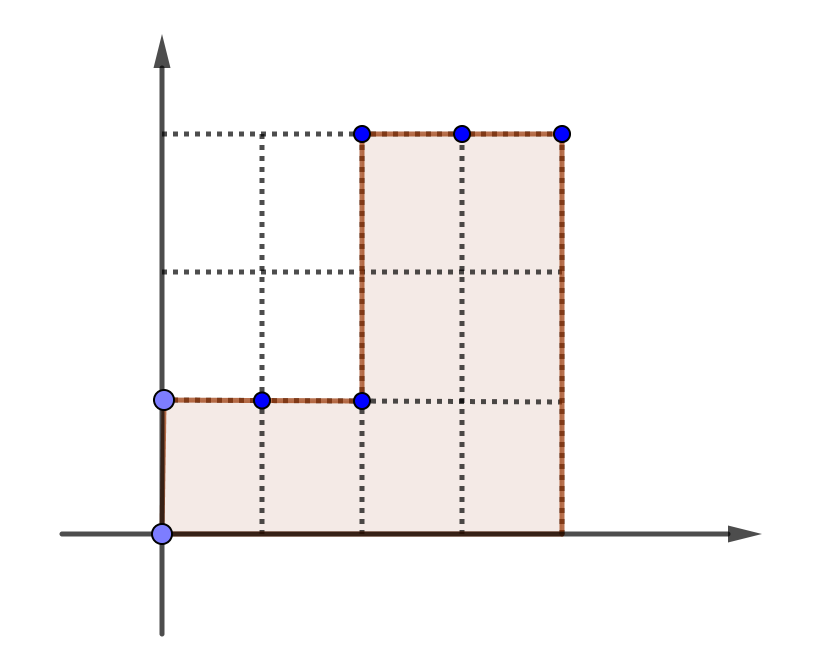
\includegraphics[width=.4\paperwidth]{roc_auc2.png}
		\end{center}
		
		Профит, получили roc-кривую.  Видим, что площадь под ней равна $\frac{8}{12}$. Иным языком говоря, среди $12$ пар ноликов и единичек, вероятности отсортированы так, как нам хотелось бы $8$ раз. 
		
		Для первого наблюдения $(1, 0.9)$ все четыре пары верны. Для второго $(1, 0.56)$ будет одна ошибочная сортировка, для третьей $(1,0.2)$ будет три ошибочных сортировки. 
	\end{enumerate}
\end{solution}

\todo[inline]{Задачки ниже --- новые}  

\begin{problem}
Алгоритм бинарной классификации, придуманный Бандерлогом, выдаёт оценки вероятности $\hat p_i = \hat P(y_i=1)$. Всего у Бандерлога $10000$ наблюдений. Если ранжировать их по возрастанию $\hat p_i$, то окажется что наблюдения с $y_i = 1$ занимают ровно места с  $5501$ по $5600$. Найдите площадь по ROC-кривой и площадь под PR-кривой.
\end{problem}

\begin{solution} 

Предположим, что у всех объектов разные вероятности и посчитаем ROC-AUC. Все единички стоят на местах с \(5501\) по \(5600\), значит в выборке есть  \(100\) единичек и \(10000-100=9900\) нулей, поэтому у нас есть \(100 \cdot 9900=990000\) пар между нулями и единичками. 

При сравнении вероятности любой единички с вероятностью любого нуля на местах с \(1\) по \(5500\), вероятность единички (вероятность того, что объект принадлежит классу с меткой 1) будет больше вероятности нуля, и это ок, и у нас будет \(100 \cdot 5500=550000\) хороших пар, где ранжирование правильное. 

Однако при сравнении вероятности любой единички с вероятностью нуля на местах, начиная с \(5601\), вероятность единички будет меньше вероятности нуля, и это не ок, должно быть наоборот. 

Поэтому если считать ROC-AUC как долю пар нулей и единичек, где ранжирование вероятностей верное, то ROC-AUC\(=550000/990000=5/9=0.556\).

Посчитаем PR-AUC. При выборе очень маленького порога мы будем считать все объекты единичками, тогда полнота будет равна \(1\), а точность – \(100/10000=1/100=0.01\).

Если мы будем повышать порог до значения вероятности единички на \(5501\)-ом месте, то полнота по-прежнему будет равна \(1\), а точность будет возрастать по мере увеличения порога: сначала будет \(100/10000\), затем – \(100/9999\), \(100/9998\), \(100/9997\), ..., \(100/4501\), \(100/4500\). 

Полнота начнет изменяться, если порог сделать равным вероятности на \(5501\)-ом месте, тогда одну единичку мы посчитаем нулем и полнота станет равна \(99/100\). Точность изменится на значение \(99/(10000-5501)=99/4499\). Если порог сделать равным вероятности на \(5502\)-ом месте, то мы посчитаем 2 единички нулями, и полнота снизится до \(98/100\), а точность до \(98/4498\).

Так пара полноты и точности будут меняться следующим образом: (\(100/100\), \(100/4500\)), (\(99/100\), \(99/4499\)), (\(98/100\), \(98/4498\)), ..., \((1/100\), \(1/4401\)), (\(0/100\), \(0/4400\)). В конце, когда мы сделаем порог равным вероятности нолика на \(5601\)-ом месте мы получим нулевую полноту и точность.

Таким образом, в качестве PR-кривой можно нарисовать прямую линию между точками (\(0,0\)) и (\(1, 100/4500\)), площадь под которой равна \(0.5 \cdot1 \cdot  (100/4500)=50/4500=1/90=0.0111\).

\end{solution} 


\begin{problem}
Для задачи классификации есть довольно много разных метрик, которые оценивают качество модели для её решения. На практике иногда оказывается, что по одной метрике наша модель может иметь более высокое качество, чем другая, а по другой метрике --- более низкое. 

Предположим, что у нас есть две модели, предсказывающие принадлежность к одному из классов: котики, $1$ или собачки, $0$. Качество моделей оценивается на выборке из пяти объектов.  
Оказывается, что по метрике $A$ первая модель лучше, а по метрике $B$, вторая. Вам нужно придумать примеры тестовых меток $y$ и предсказаний $\hat y_1$ и $\hat y_2$ для каждой пары метрик $A$ и $B$: 

\begin{enumerate} 
\item[а)] A --- precision (при пороге $0.5$), B --- auc-roc;

\item[б)] A --- precision (при пороге $0.5$), B --- recall (при пороге $0.5$);

\item[в)] A --- F1-score (при пороге доставляющем максимум), B --- auc-roc.
\end{enumerate} 
\end{problem} 


\begin{solution} 
В решении просто примеры подобных меток и прогнозов. Понятное дело, что у задачки нет одного решения. 
\begin{enumerate}

	\item Пусть $y = (1,1,1,0,0)$. Для первого алгоритма $\hat p_A = (0.95, 0.8, 0.8, 0.9, 0.7)$. Для второго алгоритма $\hat p_B = (0.7, 0.8, 0.3, 0.9, 0.4)$. Порог $0.5$. Всего у нас $6$ пар классов. Видим, что для первого алгоритма ROC-AUC составит $\frac{4}{6} = 0.66$. Для второго ROC-AUC составит $0.33$.  Посчитаем точность. Для первого она составит $0.6$. Для второго $0.66$. Видим, что второй алгоритм лучше по точности. Первый лучше по ROC-AUC. 
	
	\item  Пусть $y = (1,1,1,0,0)$. Для первого алгоритма $\hat p_A = (0.9, 0.8, 0.8, 0.8, 0.8)$. Для второго $\hat p_B = (0.8,0.8,0.4,0.4,0.8)$.  Порог $0.5$. Для первого алгоритма все прогнозы единичные. Точность составит $0.6$. Полнота составит $1$. Для второго алгоритма одна единица выпадает из прогнозирования и один ноль. Точность составит $0.66$.  Полнота составит тоже $0.66$. Видим, что первый алгоритм оказался лучше по полноте, второй оказался лучше по точности.  
	
	\item  Пусть $y = (1,1,1,1,0)$. Для первого алгоритма $\hat p_A = (1,1,1,0,1)$. Для второго алгоритма $\hat p_B = (1,1,1,1,1)$. Тогда Для первого алгоритма $ROC-AUC = 0.75$. Для второго $ROC-AUC = 0.5$. В случае f-меры получаем обратную картину. В первой ситуации $f = 2 \cdot \frac{0.75 \cdot 0.75}{0.75 + 0.75} = 0.75$ для любого порога. Во второй ситуации получаем $2 \cdot \frac{0.8 \cdot 1}{0.8 + 1} =0.88$. 
\end{enumerate}
\end{solution}

\todo[inline]{Задачу ниже перепроверить}

\begin{problem} 
Винни-Пух пришёл в лесу к власти у становил свою медвежью диктатуру. Верные Винни-Пуху медведи случайно рассредоточились по лесу и обнюхивают его. Их главная задача --- поиск правильных пчёл для изъятия у них мёда. После каждого изъятия медведи записывают в книжечку всех пчёл и обстоятельства, в которых они были найдены. 

В один прекрасный день Винни-Пух решил обучить классификатор для поиска правильных пчёл. Он это сделал на сбалансированной обучающей выборке (взял по $5000$ плохих и хороших пчёл), а после на сбалансированной тестовой выборке (по $500$ пчёл) он посчитал метрики качества. 

\begin{enumerate} 
\item[а)] В качестве порога Винни взял $0.5$. Точность (precision) получилась $0.9$. Полнота (recall) получилась $0.7$. Как выглядит матрица ошибок (confusion matrix)? 

\item[б)] В природе всего лишь $10\%$ пчёл правильные. Медведи зашли в гости к случайной $1000$ пчёл. Сколько из них классификатор назовёт правильными? Сколько раз он ошибётся? Нарисуйте для это выборки матрицу ошибок и найдите precision и recall. 

\item[в)] Правда ли, что ни precision ни recall не поменялись при переходе от сбалансированной тестовой выборки к природной? Как сделать так, чтобы на практике не задумываться о таких переходах? 

% \item[г)] Что будет происходить при таком переходе от сбалансированной выборки к несбалансированной с ROC AUC и c PR AUC? 
\end{enumerate} 
\end{problem} 

\begin{solution}
\begin{enumerate} 
\item[а)] Для начала занесём в матрицу ошибок всю информацию, которая нам известна из условия задачи. Объектов $0$ и $1$ класса в выборке было по $500$ штук. Добивим строчку с этим числом. 

\begin{center}
    \begin{tabular}{|c|c|c|}
    	\hline
    	& $y=0$  &  $ y = 1$  \\  \hline 
    	$\hat y = 0$  & &  \\      \hline 
    	$\hat y = 1$ & &   \\ \hline 
         	& $500$ & $500$ \\ \hline 
    \end{tabular}
\end{center} 

Полнота получилась $0.7$. Это означает, что из $500$ правильных пчёл модель нашла $0.7 \cdot 500 = 350$. Выходит, что остальные $150$ она найти не смогла. Добавляем эту информацию в табличку. 

\begin{center}
    \begin{tabular}{|c|c|c|}
    	\hline
    	& $y=0$  &  $ y = 1$  \\  \hline 
    	$\hat y = 0$  & & $150$ \\      \hline 
    	$\hat y = 1$ & &  $350$ \\ \hline 
         	& $500$ & $500$ \\ \hline 
    \end{tabular}
\end{center} 

Точность оказалась $0.9$. Найдём сколько лишних пчёл модель сочла правильными: 

\begin{equation*}
\begin{aligned}
&\frac{350}{350 + x} = 0.9 \\
&0.9 \cdot x = 350 - 0.9 \cdot 350 \\
&x = 39
\end{aligned}
\end{equation*}

Можем заполнить оставшиеся две клетки.

\begin{center}
    \begin{tabular}{|c|c|c|}
    	\hline
    	& $y=0$  &  $ y = 1$  \\  \hline 
    	$\hat y = 0$  & $461$ & $150$ \\      \hline 
    	$\hat y = 1$ & $39$ &  $350$ \\ \hline 
         	& $500$ & $500$ \\ \hline 
    \end{tabular}
\end{center} 

\item[б)] В природе правильные только $10\%$ пчёл. То есть из $1000$ пчёл, к которым зашли медведи $900$ окажется неправильных. Заполним в табличке последнюю вспомогательную строку: 

\begin{center}
    \begin{tabular}{|c|c|c|}
    	\hline
    	& $y=0$  &  $ y = 1$  \\  \hline 
    	$\hat y = 0$  &  &   \\      \hline 
    	$\hat y = 1$ &  &    \\ \hline 
         	& $900$ & $100$ \\ \hline 
    \end{tabular}
\end{center} 

Начинаем размышлять. Полнота была $0.7$ Мы считали её только по объектам из $1-$го класса. Это означает, что среди $100$ правильных пчёл медведи найдут только $70$.

\begin{center}
    \begin{tabular}{|c|c|c|}
    	\hline
    	& $y=0$  &  $ y = 1$  \\  \hline 
    	$\hat y = 0$  &  & $30$  \\      \hline 
    	$\hat y = 1$ &   &  $70$   \\ \hline 
         	& $900$ & $100$ \\ \hline 
    \end{tabular}
\end{center} 

С точностью возникает проблема. Если бы у нас в выборке было бы $200$ пчёл, при этом $100$ из них были бы плохие, мы бы оказались в ситуации со сбалансированной выборкой. Тогда бы мы $10$ неправильных пчёл обозвали правильными (точность $0.9$). Но у нас в выборке $900$ неправильных пчёл. Получается, что в каждой сотне мы будем допускать $10$ ошибок. То есть всего ошибок будет $90$ штук. 

\begin{center}
    \begin{tabular}{|c|c|c|}
    	\hline
    	& $y=0$  &  $ y = 1$  \\  \hline 
    	$\hat y = 0$  & $810$  & $30$  \\      \hline 
    	$\hat y = 1$ & $90$ &  $70$   \\ \hline 
         	& $900$ & $100$ \\ \hline 
    \end{tabular}
\end{center} 

Получается, что Recall никак не изменится и останется равен $0.7$. Точность составит $70/160 \approx 0.43$.

\item[в)] Нет, это неправда. С Recall действительно не произойдёт никаких неприятностей. Precision при этом падает. Чтобы избежать такой путаницы на практике, нужно следить за тем, чтобы в тестовой выборке классы соотносились друг с другом также как в природе. То есть если делается классификатор правильлных пчёл, надо понимать как часто они встречаются в природе. 
\end{enumerate} 
\end{solution}

\begin{problem} 
Настя модерирует классификатор спама. Ей хочется понять когда он устареет, испортится и надо будет научить новый. Каждый день она берёт $100$ забаненных наблюдений и $100$ не забаненных, размечает их, рисует матрицу ошибок и считает по ней Precision и Recall. Правда ли, что у Насти получится таким образом адекватно оценить эти две метрики? 
\end{problem} 

\begin{solution}
Это полуправда. Всомним как выглядит матрица ошибок: 

\begin{center}
	\begin{tabular}{|c|c|c|}
		\hline
		& $y=0$  &  $ y = 1$ \\  \hline 
		$\hat y = 0$ & $TN$ & $FN$ \\ \hline 
		$\hat y = 1$ & $FP$ & $TP$ \\ \hline
	\end{tabular}
\end{center}

Когда Настя берёт $100$ забаненных статей, она срезает строчку $\hat y = 1$. Она может сделать это, так как знает все вердикты классификатора. Когда она их разметит, она сможет адекватно понять чему равны $FP$ и $TP$, а после оценить точность классификатора спама. \indef{С Precision всё в порядке.} 

Для того, чтобы оценить Recall Насте необходимо делать срез по столбцу, где $y=1$. Реальные $y$ Настя не знает. Чтобы узнать их, ей придётся разметить всю выборку. Из-за этого будут возникать ситуации, когда у Насти не получится адекватно оценить Recall по сотне наблюдений. 

Настя делает в своей процедуре срез по строке $\hat y = 0$. Если в природе классы $0$ и $1$ встречаются одинаково часто (сбалансированно), Настя сможет оценить Recall. Если класса $0$ на порядок больше, чем класса $1$, для оценки Recall ей придётся сделать очень большую выборку по этому срезу. Например, если спам встречается только в $1\%$ статей, сотни наблюдений явно не хватит. \indef{С Recall у Насти будут проблемы.}  
\end{solution}

\begin{problem} 
Винни-Пух наладил с бандерлогами торговлю мёдом. Бандерлоги любят мёд. Многие Бандерлоги стали постоянными клиентами Винни-Пуха. Иногда Бандерлогам надоедает мёд Винни-Пуха, они начинают унывать и отваливаются от его постоянной клиентуры. 

Ситуация, когда Бандерлоги унывают называется \indef{оттоком.} Чтобы бороться с ним, Винни-Пух позвал медведей-аналитиков и вместе они обучили классификатор, который прогнозирует вероятность оттока для каждого конкретного Бандерлога. Винни попробовал посмотреть что будет происходить с моделью при двух разных порогах ($0.5$ и $0.8$): 


\begin{minipage}[t]{0.45\textwidth}
\begin{center} 
	\begin{tabular}{|c|c|c|}
		\hline
		& $y=0$  &  $ y = 1$ \\  \hline 
		$\hat y = 0$  &   $70$ &    $10$ \\      \hline 
		$\hat y = 1$ &   $20$ &    $30$ \\      \hline
	\end{tabular}
\end{center} 
\end{minipage}
\begin{minipage}[t]{0.45\textwidth}
\begin{center} 
	\begin{tabular}{|c|c|c|}
		\hline
		& $y=0$  &  $ y = 1$ \\  \hline 
		$\hat y = 0$  &   $80$ &    $20$ \\      \hline 
		$\hat y = 1$ &   $10$ &    $20$ \\      \hline
	\end{tabular}
\end{center} 
\end{minipage}


Один горшочек мёда стоит $100\$$. Если модель спрогнозировала отток, Бандерлогу будет даваться скидка в $10\%$. Средний доход от одного Бандерлога за месяц составляет $300\$$. С помощью тестовой выборки ответьте на следующие вопросы:  

\begin{enumerate} 
\item[а)] Сколько баксов мог бы заработать Винни за месяц, если бы никто из Бандерлогов не уходил? Сколько баксов потерял бы Винни, если бы он давал бы Бандерлогам спокойно уходить? 

\item[б)] Сколько баксов для обеих моделей Винни потратит на скидки? Сколько баксов будет потрачено впустую? Какой суммарный средний доход Винни сможет удержать благодаря модели? Выгодно ли это?  

\item[в)] Придумайте на основе всех этих расчётов бизнес-метрику, на основе которой Винни-Пух мог бы выбрать порог для своей модели. 

\item[г)] Как правильно выкатить такую модель в продакшн (включить работать в режиме реального времени) так, чтобы никто не пострадал? 
\end{enumerate} 
\end{problem} 

\begin{solution}
\begin{enumerate} 
\item[а)] Всего есть $130$ Бандерлогов. Каждый в среднем приносит $300\$$. Если бы из тестовой выборки от нас никто не уходил, мы бы заработали $130 \cdot 300 = 39000\$$.

Если бы Винни ничего не делал, от него бы ушли $40$ Бандерлогов. Получается он потерял бы  $40 \cdot 300 = 12000\$$.

\item[б)] \textbf{В первой модели} Винни дал скидку $20 + 30 = 50$ Бандерлогам. Для каждого в среднем скидка составила $0.1 \cdot 300 = 30\$$. Всего было недополучено $30 \cdot 50 = 1500\$$. Целых $20$ бандерлогов получили скидку зря. 

Из тех, кто хотел уйти, $10$ ушли. На них Винни потерял $3000$ потенциальных долларов. Если все $30$ желающих уйти, после предоставления скидки останутся клиентами Винни (что далеко не факт),  Винни потеряет $3000 + 1500 = 4500\$$. По сравнению с $12000\$$ в ситуации, когда никаких действий по удержанию не предпринимается, это неплохо.

\begin{center} 
\begin{tabular}{|c|c|c|}
	\hline
	& $y=0$  &  $ y = 1$ \\  \hline 
	$\hat y = 0$  &   $0$ &    $-3000$ \\      \hline 
	$\hat y = 1$ &   $-600$ &  $-900$ \\      \hline
\end{tabular}
\end{center} 

\textbf{Во второй модели} Винни дал скидку $10 + 20 = 30$ Бандерлогам. Из-за этого он не дополучил $30 \cdot 30 = 900\$$.  Зря получили скидку $10$ бандерлогов ($300\$$). 

Из тех, кто хотел уйти, ушло $20$. Это $6000\$$. Если удержанные $20$ останутся, потери составят $6000 + 900 = 6900\$$. Это явно больше, чем при первом выборе порога. 

\begin{center} 
\begin{tabular}{|c|c|c|}
	\hline
	& $y=0$  &  $ y = 1$ \\  \hline 
	$\hat y = 0$  &   $0$ &    $-6000$ \\      \hline 
	$\hat y = 1$ &   $-300$ &  $-600$ \\      \hline
\end{tabular}
\end{center} 

\item[в)] Пришло время превратить наши расчёты в бизнес-правило для выбора порога. Давайте занесём все действия, которые мы можем предпринять и денежные потери в табличку. Пусть $sale$ это скидка, а $RPU$ среднемесячный доход: 

\begin{minipage}[t]{0.45\textwidth}
\begin{center} 
	\begin{tabular}{|c|c|c|}
		\hline
		& $y=0$  &  $ y = 1$ \\  \hline 
		$\hat y = 0$  &   $TN$ &    $FN$ \\      \hline 
		$\hat y = 1$ &   $FP$ &    $TP$ \\      \hline
	\end{tabular}
\end{center} 
\end{minipage}
\hfill
\begin{minipage}[t]{0.45\textwidth}
\begin{center} 
    \begin{tabular}{|c|c|c|c|}
    	\hline
    	& $y=0$  &  $ y = 1$  & действие\\  \hline 
    	$\hat y = 0$  &  $0$ &   $-RPU$ & ничего \\ \hline 
    	$\hat y = 1$ &   $-sale$ & $RPU - sale$ & скидка \\ \hline
    \end{tabular}
\end{center} 
\end{minipage}

Тогда наша бизнес-метрика будет такой: 

$$
(RPU - sale) \cdot TP  - sale \cdot FP - RPU \cdot FN \to \min_{\text{выбор порога}} 
$$

Винни-Пух попробовал только два значения порога. Нам нужно перебрать их все. Где наши потери будут минимальными, тот порог нам подойдёт лучше всего.   

Помните $f-$меру? Она тоже пыталась сочетать в себе разные ошибки из нашей таблички, но никак не взвешивала их на деньги. Текущая метрика взвешивает. Из-за этого мы можем принимать решения более релевантные для нашего бизнеса.  Как обычно, есть нюансы:

\begin{itemize}
    \item Каждый раз, когда мы делали подсчёт денег, которые нам в среднем удастся сохранить, мы говорили важные слова: \indef{если удержанные останутся.} Вообще не факт, что люди после предоставления скидки захотят остаться нашими клиентами. Вероятность того, что они всё-равно уйдут, по-прежнему очень высока. По хорошему, нам нужно немного изменить нашу метрику: 
    
$$
P(\text{скидка помогла}) \cdot (RPU - sale) \cdot TP  - sale \cdot FP - RPU \cdot FN
$$

Откуда раздобыть вероятность того, что скидка поможет --- очень большой вопрос. Можно схитрить и попробовать как-то задействовать здесь уверенность нашей модели в её прогнозе, либо провести какие-то дополнительные исследования, которые помогут нам эту вероятность оценить, и сделать её для всех людей одинаковой. На самом деле этот финт тоже не очень честный, вероятность очень индивидуальна. 

\item Можно перебирать не только пороги для модели, но ещё и размеры скидки. Более того, чем больше скидку мы дадим, тем выше будет $P(\text{скидка помогла})$. Это подливает масла в огонь неопределённости. Машинное обучение, несмотря на свою красоту, довольно неточная наука. 
\end{itemize}

\item[г)]  Посмотреть на тестовую выборку и посчитать цифры из предыдущих пунктов --- недостаточно. Картина будет довольно сильно искажена. Как минимум из-за того, что мы не знаем вероятности того, что человек, который хотел уйти, останется в нашем магазине после предоставления скидки. А ещё не знаем как скидка влияет на эту вероятность. 

Перед тем, как начать применять модель в реальной жизни, надо \indef{провести АБ-тест.} Для этого мы возьмём $1\%$ пользователей, для которых будем применять модель. Для остальных всё оставим по старому. Подождём пару месяцев. 

После мы сможем посчитать долю оттока в группе, где модель применялась и долю оттока, где она не применялась. Если эти доли окажутся \indef{значимо разными,} модель можно применять на более широкую аудиторию. 

Такой тест может заодно помочь оценить вероятность того, что скидка помогла и немного откорректировать выбор порога. Правда тогда придётся провести новый АБ-тест. 

С АБ-тестами тоже есть проблемы. Если их неправильно проводить, можно напороться на разные ложные связи. Про них разговор пойдёт немного позже. Чтобы делать всё правильно, нужно будет выучить теорию вероятностей и матстат. Отнеситесь к этим дисциплинам серьёзно. Они правда нужны в жизни.  
\end{enumerate} 
\end{solution}


\end{document}
